\section{Datenaufbereitung und Sensorfusion}

Abbildung~\ref{fig:pipeline} gibt einen Überblick über die gesamte Verarbeitungskette. Die einzelnen Schritte werden in den folgenden Abschnitten detailliert beschrieben.

\begin{figure}[H]
\centering
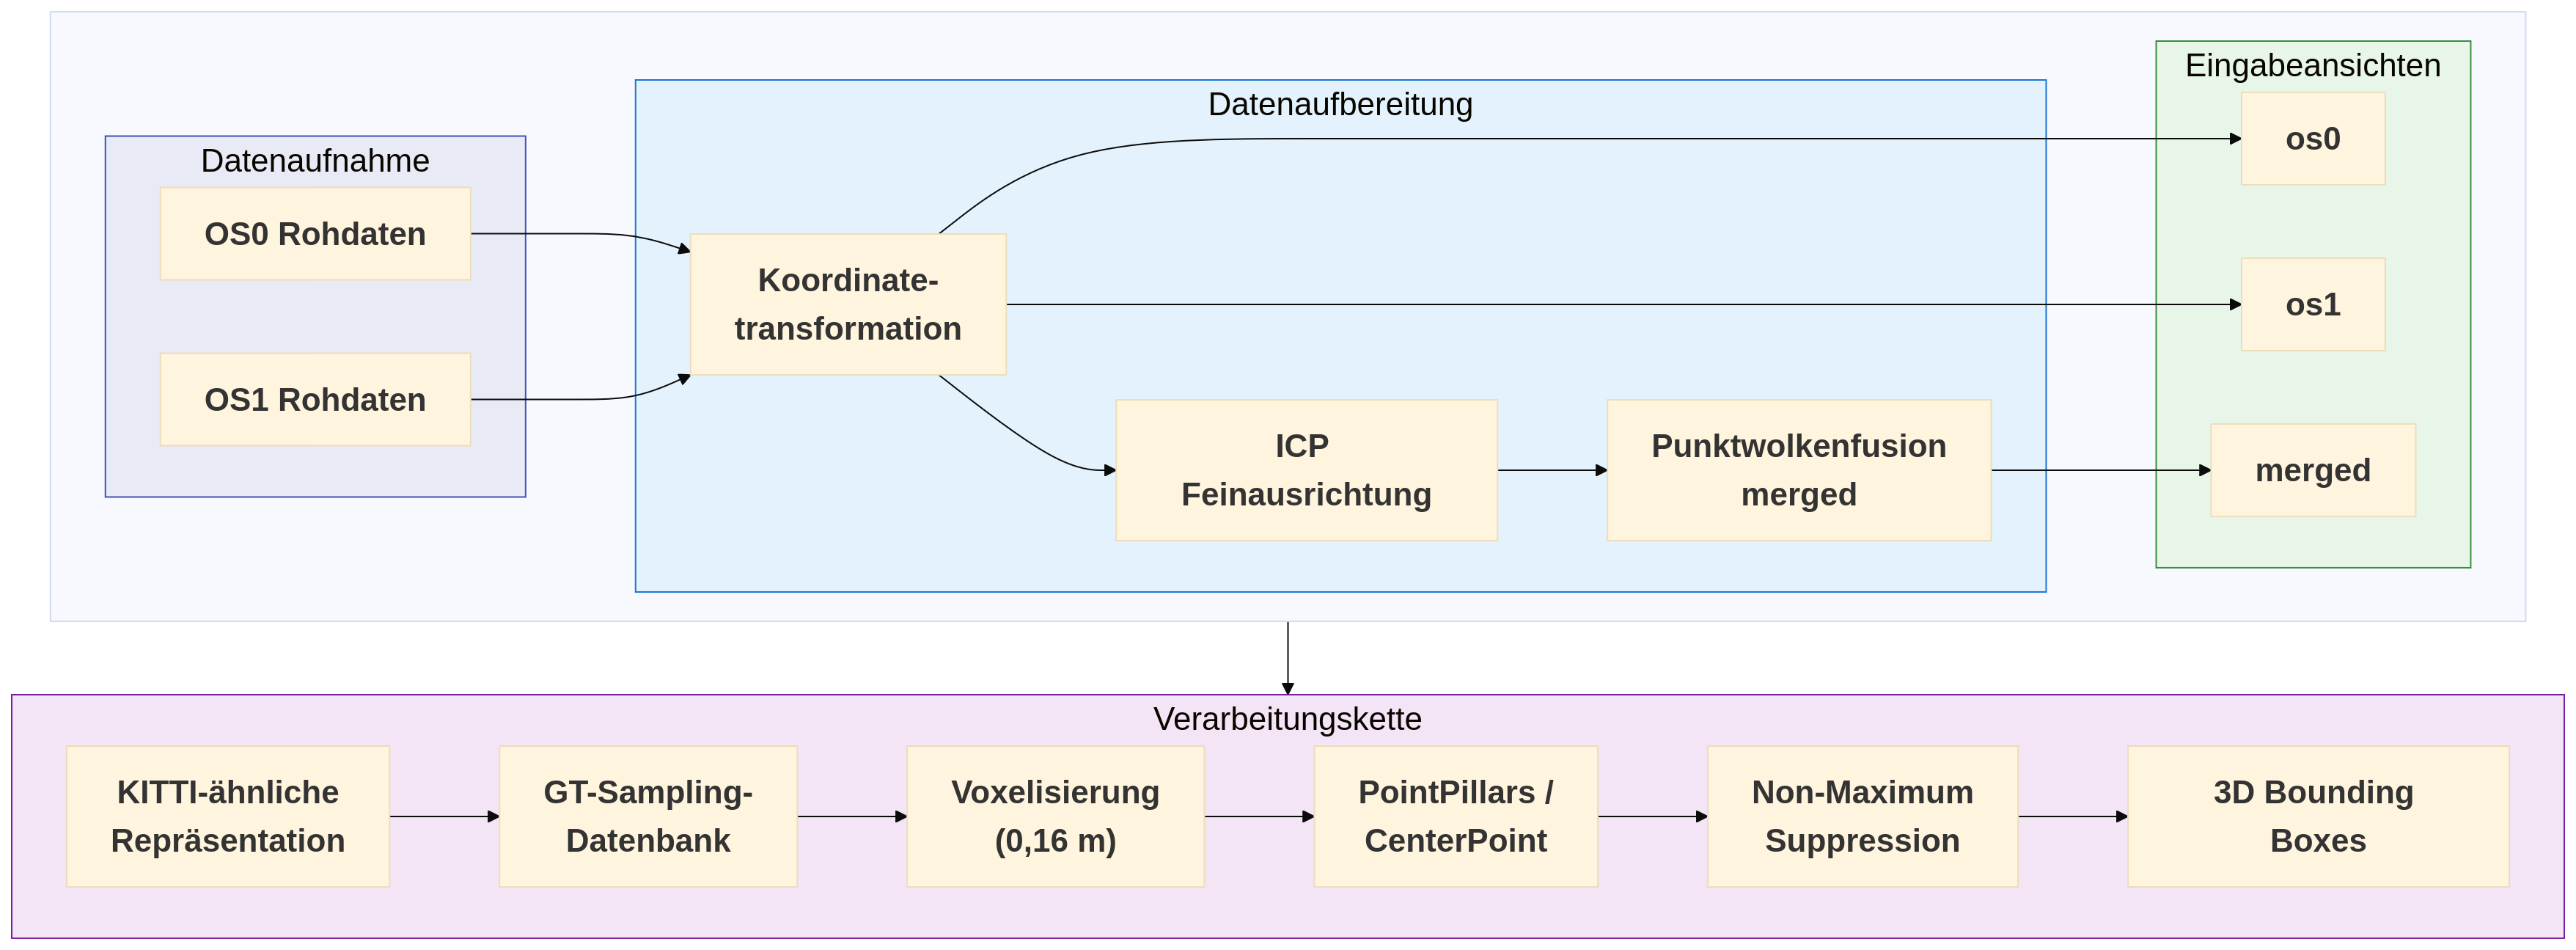
\includegraphics[width=\textwidth]{images/pipeline-diagram.png}
\caption{Verarbeitungskette von den Rohdaten über Fusion und Augmentierung bis zur 3D-Box-Prädiktion.}
\label{fig:pipeline}
\end{figure}

\subsection{Registrierung und Merge}

Die Merge-Pipeline ist in \texttt{experiment/pcd\_merge.py} implementiert. Sie führt für jedes Sensorpaar folgende Schritte aus:

\begin{enumerate}
    \item Laden der beiden Punktwolken und ihrer Intensitätswerte,
    \item Entfernen statistischer Ausreißer,
    \item Anwenden einer manuell bestimmten Vorabtransformation,
    \item Voxel-Downsampling und Normalenschätzung,
    \item Feinausrichtung durch Iterative Closest Point (ICP) \cite{besl1992icp},
    \item Konkatenation der transformierten Punkte.
\end{enumerate}

Die beiden Sensoren sind fest montiert. Für einen späteren Online-Betrieb wäre deshalb eine einmalig auf einer geeigneten statischen Szene bestimmte Extrinsik vorzuziehen. Die aktuelle Implementierung berechnet die ICP-Korrektur dagegen für jeden Frame neu. Das ist für die Offline-Erzeugung der Projektdaten verwendbar, aber weder laufzeitoptimal noch als endgültige Live-Pipeline zu verstehen.

\subsection{Konvertierung in das Trainingsformat}
\label{sec:konvertierung}

MMDetection3D \cite{mmdet3d2020} verarbeitet die Daten in einer KITTI-ähnlichen Repräsentation \cite{geiger2012kitti}. Eigene Converter übertragen Punktwolken und Labels in dieses Format und erzeugen die benötigten Info-PKLs. Dabei wurden mehrere geometrische und metrische Fehler identifiziert und korrigiert:

\begin{itemize}
    \item \textbf{Abgeschnittener Boden.} Der Boden lag durch eine fehlerhafte \(z\)-Transformation außerhalb des vorgesehenen Punktwolkenbereichs. Dem Training fehlten dadurch der Boden und die unteren rund 40\,cm aller Objekte.
    \item \textbf{Schwebende Boxen.} Der Label-Editor speichert die \(z\)-Koordinate im Boxzentrum, während die Trainingspipeline an einer Stelle die Boxunterkante erwartete. Ohne Korrektur saßen die Boxen um eine halbe Objekthöhe, also ungefähr 75\,cm, zu hoch.
    \item \textbf{Nicht vergleichbare Intensitäten.} Intensitäten wurden ursprünglich frameabhängig normiert, sodass dieselbe Oberfläche je Aufnahme andere Werte erhielt. Sie werden nun mit einer festen Skala verarbeitet.
    \item \textbf{Verzerrte Metrik.} Die frühere Metrik mittelte AP pro Frame und wertete Frames ohne Instanz der betrachteten Klasse als Null. Da Fahrräder nur in einem Teil der Frames vorkommen, war die erreichbare Fahrrad-AP dadurch nach oben gedeckelt. Die aktuelle Implementierung berechnet datensatzweite AP.
\end{itemize}

Der Metrikfehler war der folgenreichste der vier Punkte, weil er nicht das Modell, sondern dessen Bewertung betraf: Auf identischem Modelloutput steigt der Fahrrad-AP\textsubscript{30} von 0{,}24 auf 0{,}94, sobald datensatzweit statt frameweise gemittelt wird. Aufgefallen ist der Fehler, weil zwei unterschiedlich trainierte Modelle exakt denselben Fahrradwert erreichten -- genau das Maximum, das die fehlerhafte Rechnung überhaupt zulässt. Das fehlerhafte Vorgehen hat die Modellqualität also nie verschlechtert, sondern nur verdeckt.

Alle in diesem Bericht genannten Leistungszahlen basieren auf dem korrigierten Datenstand. Frühere absolute Werte, die mit abgeschnittenem Boden, verschobenen Boxen oder der fehlerhaften Pro-Frame-Metrik entstanden sind, wurden verworfen und werden nicht berichtet.

Davon zu unterscheiden sind die in den Abschnitten~\ref{sec:gtsampling} und \ref{sec:ursachen} herangezogenen Ablationen. Sie stammen aus einer früheren Projektphase und dienen ausschließlich dem relativen Vergleich zweier Konfigurationen, die jeweils unter identischen Bedingungen trainiert wurden. Ihre Richtungsaussagen werden hier verwendet, ihre absoluten Werte nicht. Auf welchem Datenstand die Ablationen im Einzelnen gelaufen sind, ist im Bericht nicht durchgängig dokumentiert; eine Wiederholung auf dem korrigierten Stand steht aus.
